\cotefile{131}
\scanpage{2}
\mspage{A}
\margin{\unsure{conditions} \unsure{d'exactitude}}
\margin{\figure{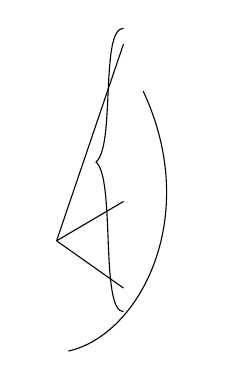
\begin{tikzpicture}[x=1cm,y=1cm]
\draw (1,3.6) .. controls (.7,3.6) and (.9,2.1) .. (.65,1.9) .. controls (.9,1.7) and (.7,0) .. (1,0);
\draw (.15,.9)--(1,3.4) (.15,.9)--(1,1.4) (.15,.9)--(1,.3);
\node at (-.1,.3) {$\varprojlim$};
\draw (1.25,2.8) .. controls (2,1.2) and (1.2,-.3) .. (.3,-.5);
\node at (0,-.5) {$\varinjlim$};
\end{tikzpicture}}}

$1^\circ$ $F$ faisceau pour la top \unsure{fppc|fpqc}
\margin{$\left\{\begin{array}{l}
\text{a) de nature locale Zariski}\\
\text{b) compatible aux \unsure{changts} \unsure{fid.}}\\
\text{\unsure{plt} \unsure{par.} \unsure{qcts} affines}
\end{array}\right.$}

$2^\circ$ $F$ commute aux $\varinjlim$ d'anneaux
\margin{(propriété \uline{relative})}

$3^\circ$ $F$ commute aux $\varprojlim$ adiques d'anneaux \uuline{\uline{artiniens}}

$4^\circ$ Pour tout anneau artinien $A$ sur $S$, $F_{\unsure{A}}$ est exact à \unsure{g.} sur la catégorie des \unsure{algèbres} \deleted{artiniens} finies sur $A$ (ou aussi, une suite exacte
\[
 A\longrightarrow A'\rightrightarrows A'\otimes_A A'=A''
\]
\inserted{$A$ artinien local}
\deleted{d'anneaux artiniens}, avec $A'\deleted{A''}$ \unsure{finis} sur $A$,
\inserted{[ext. résiduelle triviale, $\operatorname{long}_A A'/A=1$]}
donne une suite exacte
\[
 F(A)\mathrel{\unsure{-|\longrightarrow}}F(A')\rightrightarrows F(A'')
\]
].

\margin{\uline{finitude} \uline{ou} \uline{discrétion}}
\margin{\unsure{pour} \unsure{assurer|aux} \unsure{foncteurs} \unsure{sur} $X/k$\quad
$F(k)\xrightarrow{\sim}F(X)$ \unsure{pour} \unsure{v.} \unsure{(de t.f. sur k)}\quad
\unsure{n'induit aucune} \unsure{f.}\quad (\unsure{ou :} $X$ intègre)}
$5^\circ$ \deleted{\unsure{F séparé}} Pour tout anneau \deleted{\unsure{local}} \deleted{\unsure{complet}} \inserted{corps alg clos} $K$ sur $S$, et $\forall\ \xi\in F(K)$, l'anneau $B$ sur $K$ qui proreprésente $F_K$ en $\xi$ est \uline{fini} sur $K$.
\margin{(propriété \uline{relative})}

\margin{\uline{séparation}}
$6^\circ$ $F$ est \uline{séparé} sur $S$
\inserted{(par critère valuatif)}
\margin{(propriété \uline{relative})}

\margin{critère de \uline{modularité}\quad a) \uline{locale}}
$7^\circ$ Pour tout $S'$ local noeth complet, \inserted{sur $S$} $\forall\ t\longrightarrow Z$ \inserted{local} fini sur $S$, pt fermé $t$, \deleted{\unsure{a}}
\unsure{tout} $\unsure{\eta|y}:Z\longrightarrow F_{S'}$ [$\simeq\unsure{\eta|y}\in Z\mathrel{\unsure{-|\longrightarrow}}F$]
qui est \unsure{modulaire} (pour $F_{S'}$) au pt fermé $t$ de $Z$, $\unsure{\eta|y}$ est \unsure{modulaire} \inserted{[ou tout au moins, étale]} en tout point.
\diagram{\begin{tikzcd}
F\arrow[d] & F_{S'}\arrow[l]\arrow[d] & \\
S\arrow[r,no head] & S' & Z\arrow[l]\arrow[ul,"\unsure{\eta|y}"']
\end{tikzcd}}
\margin{On peut supposer $S'$ \unsure{irréductiblement} de dim $1$ (et $\unsure{F_{s'_0}|F_{s'}}$ représentable, \unsure{si} \deleted{\unsure{sur} $S'$} $s'$ est le pt générique de $S'$)}

\margin{b) \uline{générique}}
$8^\circ$ Pour tout $S'$ noeth irréductible sur $S$, et $Z\mathrel{\unsure{\longrightarrow|-}}S'$ \inserted{irréductible} \uline{fini} sur $S'$, $\unsure{\eta|y}:Z\longrightarrow F_{S'}$ tel que $\unsure{\eta|y}$ soit \unsure{modulaire} pour $F_{S'}$ au pt générique $z$ de $Z$, il existe un ouvert $U\ni z$ tel que $\unsure{\eta|y}$ soit \unsure{modulaire} (ou tt au moins étale) en tt point de $U$
\mspage{1}
